\documentclass[11pt]{amsart}
\usepackage{geometry}           % See geometry.pdf to learn the layout options. There are lots.
\geometry{letterpaper}          % ... or a4paper or a5paper or ... 
%\geometry{landscape}           % Activate for for rotated page geometry
%\usepackage[parfill]{parskip} 	% Activate to begin paragraphs with an 
								% empty line rather than an indent
\usepackage{graphicx}
\usepackage{amssymb}
\usepackage{epstopdf}
\usepackage{tikz-qtree}
\usepackage{enumitem}

\DeclareGraphicsRule{.tif}{png}{.png}{`convert #1 `dirname #1`/`basename #1 .tif`.png}

\title{Proposition of Volunteer Cloud Computing}
\author{Dany Wilson}
%\date{}                                         % Activate to display a given date or no date

\begin{document}
\maketitle
	\section{Introduction}
	In this current era we can see a shift in how software and hardware are conceived, the end-
	goals are not the same as they used to be 2 decades ago. This can be attributed to the 
	following, the fact that the Internet speed got a lot faster, by a factor of 1000 (based on
	a 56kbps connection in 1995, compared to a 50mbps connection today), but also because the 
	hardware performance augmented at a similar pace. Initially in the pre-Internet era, 
	software was written to be executed locally without any network interactions. Then in the 
	genesis of the Internet, the objectives of software slowly shifted to access external 
	resources, thus the apparition of the e-mail and the web-browser. Slowly as the connection
	bandwidths increased, there was an increased number of possible usage such as online games, 
	content streaming, social-media, etc. Nowadays we can access fully virtualized computing
	environments within our web-browsers, and this takes us the very genesis of the Cloud 
	Computing era. 

	\subsection{The Genesis of Cloud Computing}
	The embodiment of Cloud Computing, namely the Internet of Things, can actually be traced 
	back to the vision of J.C.R. Licklider of the \emph{"Intergalactic Computer Network"} 
	\cite{likelider}:
	\begin{quote}
		At this extreme, the problem is essentially the one discussed by science fiction 
		writers: \emph{"how do you get communications started among totally uncorrelated 
		sapient beings?"}
	\end{quote}
	This quote shows us the state of electronic tele-communication in the sixties, which is 
	described as being fabric of fiction. There was military but also academic interest of 
	providing an infrastructure that supports long-distance information processing. One of the most 
	interesting idea of this memorandum is best conveyed in this following quote:
	\begin{quote}
		When the computer operated the programs for me, I suppose
		that the activity took place in the computer at SDC, which
		is where we have been assuming I was. However, I would just
		as soon leave that on the level of inference. With a
		sophisticated network-control system, I would not decide
		whether to send the data and have them worked on by
		programs somewhere else, or bring in programs and have them
		work on my data. I have no great objection to making that
		decision, for a while at any rate, but, in principle, it
		seems better for the computer, or the network, somehow, to
		do that.
	\end{quote}
	This very quote reflects the concept of offloading, not only of information or data, but 
	of computation as a service. In other words that in some case it would be better, given the 
	proper networking infrastructure, to offload the computation and send the data to be 
	processed remotely.
	
	Around the same time the concept of virtualization was being explored in the context of 
	mainframe computers, in order to logically divide the resources between applications 
	allowing them to run simultaneously. Throughout the years, the concept of virtualization 
	broaden and now it is possible to run a complete Operating System on the application level.
	There is a direct correlation with the coming of the virtualization of hardware and the 
	birth of the Cloud. At its very core the Cloud is use to describe the outsourcing of 
	content, resources (computing and storage), and then providing it on a "as-a-service" 
	basis or a pay-per-use model.
	
	% Need to talk about its similarities between the SOA, distributed, grid computing...
	%

	\subsection{The Cloud}
	
	% Need to address the proposed ontology of the cloud w.r.t. to Toward a Unified Ontology of Cloud 
	% Computing... (ontology.pdf)
	%
	
	Cloud Computing infrastructure offers many advantages compared to the traditional on-premise 
	infrastructure and it is why numerous companies consider outsourcing their IT infrastructure to 
	an off-premise solution. Among the most important characteristics that this type of 
	infrastructure offers, the NIST enumerates the following five \cite{nist}:
	\begin{enumerate}
		\item{\textbf{On-demand Self-service}} \emph{Consumers are not required to interact with 
		any representative of the provider to provision computing capabilities, rather it is 
		automated through the provider's infrastructure.}\\
		\item{\textbf{Broad Network Access}} \emph{Services are available over standard network 
		infrastructure and through standard	mechanisms, enabling different client platforms like 
		cell-phones, laptop, tablets, etc.}\\
		\item{\textbf{Resource Pooling}} \emph{Providers offers a pool of Resources to different 
		clients via a multi-tenant model, consisting of physical and virtual resources that can be 
		assigned and re-assigned dynamically to cater to the clients demands. Clients are only 
		aware, or able to choose the location of these resources with respect to pre-defined 
		geographical regions. }\\
		\item{\textbf{Rapid Elasticity}} \emph{Resources and services can be provisioned to scale 
		to meet the fluctuations of the client's needs at any time, at any magnitude. The provider
		offers a seemingly unlimited number of services and resources to the client.}\\
		\item{\textbf{Measured Service}} \emph{Resource usage can be monitored, controlled 
		(optimized) and reported in a manner that proves transparent to both provider and consumer.}
	\end{enumerate}
	
	In this modern day and age, among the major service providers of \emph{The Cloud} we can 
	find the likes of Google, Microsoft and Amazon, to name a few. They provide their services 
	as a three different service models:\\
	
	\begin{center}
		% Cloud Services graphic (may need to represent it better...)
		\begin{tikzpicture}
		[every tree node/.style={align=center,minimum width=\widthof{Cloud Services}}]
			\Tree 
 				[ .{Cloud Services} 
     				[ .{Software-as-a-Service\\SaaS} ]
     				[ .{Platform-as-a-Service\\PaaS} ]
     				[ .{Infrastructure-as-a-Service\\IaaS} ] ]
		\end{tikzpicture}
	\end{center}
	
	We will briefly explain each of these services in order to have a clearer picture of where 
	this proposition resides in the grand scheme of the Cloud. In order to do so we will explore 
	the question with respect of the Separation of Responsibilities, via a very concise graphical 
	depiction \cite{Blewis}:
	
	\begin{center}
		\begin{figure}[h]
			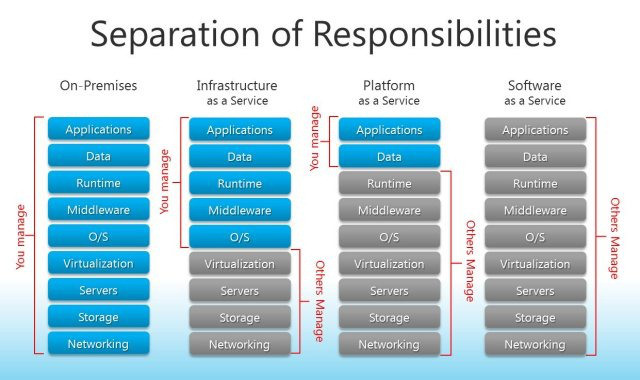
\includegraphics[width=125mm]{cloud_sep_of_resp.jpg}
			\caption{Cloud Services w.r.t. Responsibilities\label{cloud_sep_of_resp}}
		\end{figure}
	\end{center}
	
	\subsubsection{Infrastructure-as-a-Service (IaaS)}
	This service model provides, to its consumers, a virtualized environment that represents the 
	full stack, from the hardware-level to the software-level, while taking care of the hardware 
	management aspect. With this model, consumers can deploy any Operating System they wish, and as a
	matter of fact create the software environment that they deem most appropriate for their use. 
	Since the hardware management responsibility is left out to the service provider, the client can 
	easily augment or reduce the computing power at will to cope with the fluctuation of their 
	demands. Amazon's Elastic Cloud Compute (EC2), or Windows Azure are part of the available IaaS 
	solutions currently available.
	
	\subsubsection{Platform-as-a-Service (PaaS)}
	This service model, if we refer to Figure \ref{cloud_sep_of_resp}, to its clients the ability of 
	having to manage only the Application and Data aspect of the full-stack, everything else is \
	managed and taken care of by its provider. Using such a service the client can focus on simply 
	developing their application using the libraries, services and tools supported by the provider, 
	and then deploy it onto the Cloud. Google's App Engine is perhaps one of the most popular example 
	of this model.
	
	\subsubsection{Software-as-a-Service (SaaS)}
	This service model, the consumer is provided with the capability to use applications (or 
	software) running on the provider's cloud infrastructure, with little to no management 
	capability, as depicted in Figure \ref{cloud_sep_of_resp}. From a user's perspective application 
	are served as an atomic service, in the likes of Oracle ON DEMAND which offers on demand a 
	customer relationship management application.
	
	Finally we need to discuss the different \emph{Deployment Models} that are offered in the Cloud 
	eco-system. Relying again on the NIST \cite{nist} document, let's briefly present the 4 models:
	
	\begin{enumerate}
		\item{\textbf{Private Cloud}} \emph{This cloud infrastructure is meant to be used by a single 
		organization, which can act also as a single provider or a providing partner with a 3rd party 
		or solely as a consumer. Exclusivity is the key here.}\\
		\item{\textbf{Community Cloud}} \emph{Very similar to the private cloud model, but in this 
		case exclusivity of usage is shared among a community sharing common interests.}\\
		\item{\textbf{Public Cloud}} \emph{This deployment model is aimed for open use by the general 
		public, and the embodiment of this model's infrastructure is known as a Cloud Provider, such 
		as Amazon, Google, Windows, etc.}\\
		\item{\textbf{Hybrid Cloud}} \emph{This is the result of the combination of two or more 
		distinct cloud infrastructure (which remain distinct to one another), but are combined using 
		standardized or proprietary technologies to enable data and application portability.}
	\end{enumerate}

	In the following subsection we will present a fifth deployment model, namely Volunteer Cloud 
	Computing.

	\subsection{Volunteer Cloud Computing}
	The concept of Volunteer Cloud Computing is a fairly new one, since as we can see there is no 
	mention of it whatsoever in \cite{nist}\cite{taxonomy}. It revolves around user-provided 
	resources as the building components of the cloud infrastructure, and typically takes place in 
	a decentralized manner for which no single provider is designated, rather the collection of the
	participants form at the same time the provider and the consumers. One of the driving factors of 
	this topological ideology is to harvest and make efficient use of distributed idling 
	resources to provide a cloud infrastructure, with no real added cost. 
	
	In the following section we will review the literature to find out more about the position of 
	Volunteer Cloud Computing with respect to the current deployment models in place, and if any 
	implementation exists.
	
	\section{Related Work}
	
	\subsection{Cloud@Home}
	The first real apparition of the term Volunteer Cloud Computing can be attributed to 
	\cite{cathome}, in 2009 when they proposed the Cloud@Home paradigm. It can be described as a 
	continuation of the @Home distributed computing effort and the merging of volunteer computing and 
	Cloud computing. They propose an infrastructure in which it is possible for heterogeneous 
	computing resources to be connected and to co-operatively provide a Cloud infrastructure, at a 
	cost or for free. Thus this is a leap into monetizing the idle time of the consumer-grade 
	computing resources, to provide a seamless Cloud experience to consumers. Although they provide a 
	very detail analysis of the majority of the factors present in a Cloud architecture, little to no 
	information was released after the publication of a series of more specific papers on the 
	subject, %\cite{cathome2}.
	
	\subsection{P2P Cloud Architecture}
	There was other notable effort conducted with respect to this concept, albeit presented under a 
	different category one of Peer-to-peer Cloud Architecture. (cite italian paper)
	
	\section{Motivation}
	The motivation behind this proposal, is to analyze where past effort have not been has successful
	has expected. From this analysis, we wish derive a design that take on past the shortcomings of 
	the previous attempts and venture to propose a viable implementation for this paradigm, which to 
	this day seems lacking.
	
	\section{Contributions}
	In this section we will present our novel contributions with respect to previous related work.
	
	
	
	
\clearpage
\begin{thebibliography}{9}
	
		\bibitem{likelider} Licklider, J.C.R. {\emph Memorandum For: Members and Affiliates of 
		the Intergalactic Computer Network.} April 23 1963.
		
		\bibitem{nist} Mell, P., \& Grance, T. (2011). \emph{The NIST definition of cloud computing.}
		
		\bibitem{Blewis} Lewis, Brian. {\emph Taken from http://mythoughtsonit.com/2011/04/infrastructure-as-a-service-platform-as-a-service-software-as-a-servicetake-a-look-at-the-management-stack/} Consulted, November 19th 2014.
		
		\bibitem{taxonomy} Rimal, B. P., Choi, E., \& Lumb, I. (2009, August). \emph{A taxonomy and 
		survey of cloud computing systems.} In INC, IMS and IDC, 2009. NCM'09. Fifth International 
		Joint Conference on (pp. 44-51). Ieee.
		
		\bibitem{cathome} Cunsolo, V. D., Distefano, S., Puliafito, A., \& Scarpa, M. (2009). 
		\emph{Cloud@ home: Bridging the gap between volunteer and cloud computing.} In Emerging 
		Intelligent Computing Technology and Applications (pp. 423-432). Springer Berlin Heidelberg.
\end{thebibliography}

\end{document}  